\newpage
\section{Parameterisations of the negative binomial (NB1 vs NB4).}
\label{app:sec:NB1discussion}

There are at least three ways to formulate and interpret an experiment for 
the independent Bernoulli trials with a fixed number of outcomes (successes,
failures or both) with the goal to estimate its probability distribution. 
The NB model which formalises this experiment is formulated using two 
out of three following parameters dependent on the formulation: 
\begin{itemize}
\item 
number of trials (i.e. total number successes or failures) % -- usually denoted with \emph{n} or \emph{x}
\item
number of successes % -- usually denoted with \emph{n}, \emph{r} or \emph{k}
\item
number of failures % -- usually denoted with \emph{r} or \emph{k}.
\end{itemize} 
The possible formulations for such experiment are 
\begin{description}
\item[Option 1]
observing k failures before obtaining the r$^{th}$ success (most common)
\item[Option 2]
obtaining r successes until k$^{th}$ failures have occurred
\item[Option 3]
number of trials (successes or failures), $n$, required before the r$^{th}$ success occurs.
\end{description}
Option 1 is the most common formulation in the literature, see from the table \ref{figTable:NB1forms}, 
while the remaining two options are encountered only in very few cases.

The UncertML, based on the english version of Wikipedia, uses the second 
interpretation of this distribution\footnote{This was not always the case as the change 
from the standard formulation to the current one happened around 2010. The majority 
of users who commented on this change are unhappy about it, see the English and French 
Wikipedia Talk/Discussion pages. 
Because there is no agreement to reverse these changes, which would require 
significant effort, the page remains as is for the time being.}. In the current version 
of ProbOnto we have reformulated it to align with the vast majority of sources. 
Otherwise, mistake are likely as the target tools e.g. Matlab, R and 
winBUGS, to mention here only few, use the most common form, see figure 
\ref{fig:testNB}.

\begin{figure}[ht!]
\centering
  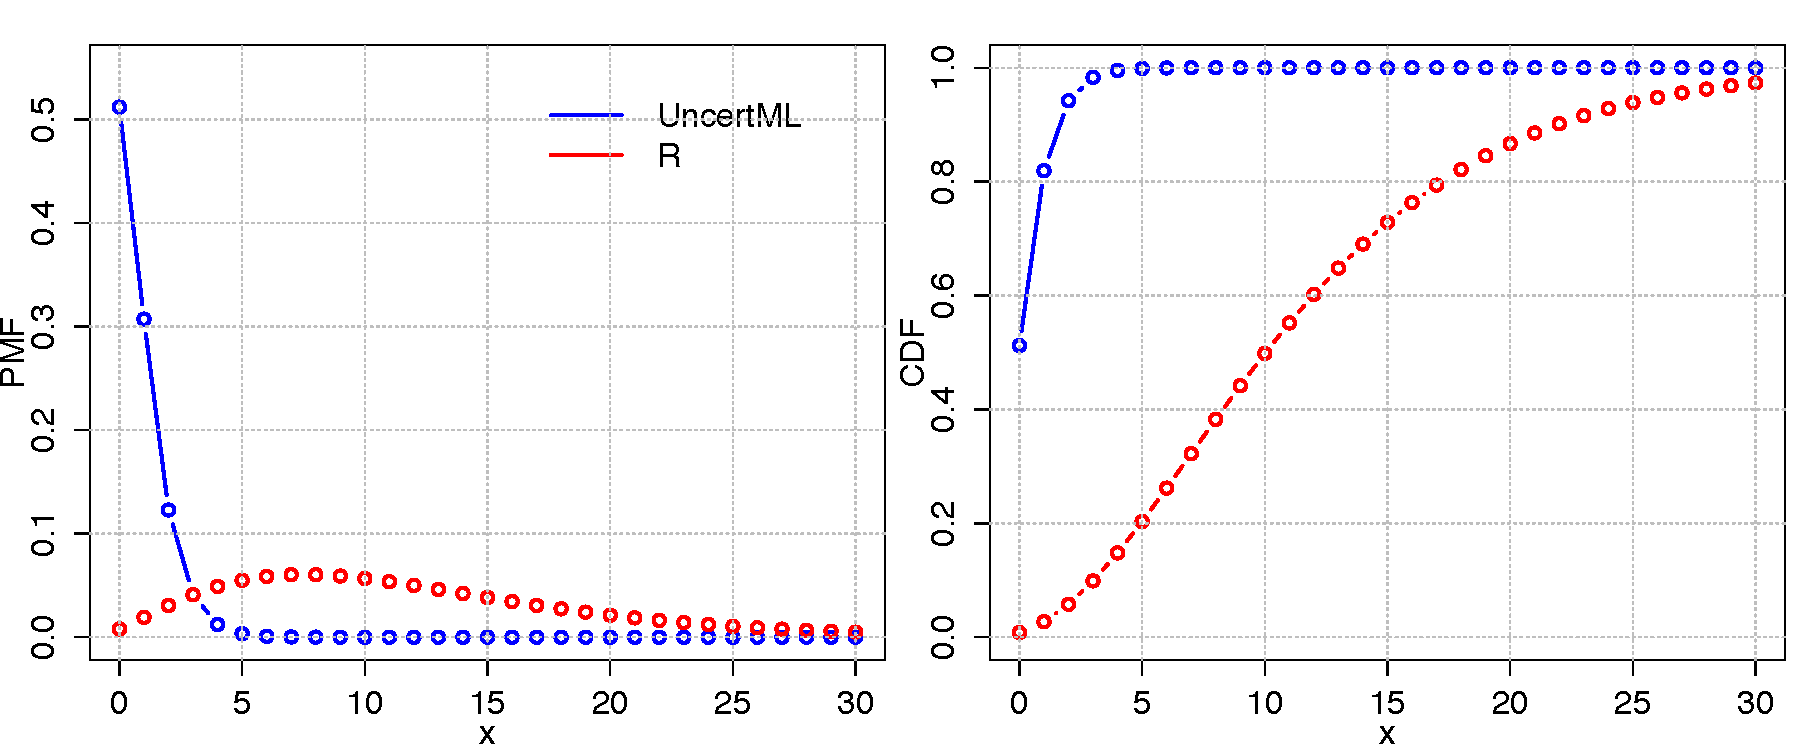
\includegraphics[width=140mm]{pics/testNB.pdf}
 \caption{Plots of the negative binomial distribution functions, 
 PMF and CDF, for the different formulations, here \emph{Option 1}
 and  \emph{Option 2} compared. In (blue) the functions
 for the UncertML formulation, in red as implemented in R for parameters 
 $r=n=3$ and $p=.2$. See table \ref{figTable:UncertMLversusR} for the 
 according PMFs and parameter definitions.}
 \label{fig:testNB}
\vspace{-1.5em}
\end{figure}

\captionsetup[longtable]{skip=1em}
\LTcapwidth=.95\textwidth
\begin{center}
\setlength{\tabcolsep}{7pt}
%\small
\renewcommand{\arraystretch}{1.1}%
\begin{longtable}{lcc}
  \hline
  \hline
  %header
   		&	UncertML								& R \\ [-0.5ex]
  \hline
  \hline
%  \multicolumn{5}{c}{\textit{Option 1}}  \\
\Gape[.4cm][0cm]{}PMF		& $f(x;r,p) = {x + r - 1 \choose x} p^x (1-p)^r$		& $f(x;n,p) = {x + n - 1 \choose x} p^n (1-p)^x$ \\
\Gape[.4cm][0cm]{}Support		& $x \in 0,1,2,...$ number of \textbf{successes} 	& $x \in 0,1,2,...$ number of \textbf{failures} \\
\Gape[.4cm][0cm]{}Parameters 	& $p \in [0,1]$ -- probability of success 			& $p \in (0,1]$ -- probability of success\\
			& $r$ -- number of \textbf{failures}				& $n$ -- number of \textbf{successes} \\
  \hline
\caption{UncertML versus R: comparison of the model formulation, parameter used
and the support variable. The mathematical formulation of the two models 
is almost identical, but because of the nuanced differences in support variable interpretation 
and meaning of the parameters, the resulting models provide very different results, 
see figure \ref{fig:testNB}.}
\label{figTable:UncertMLversusR}
\vspace{-2.5em}
\end{longtable}
\end{center}




\subsection*{Differences explained}
The above mentioned formulation options, see also table \ref{figTable:UncertMLversusR}, 
are better understood if one compares different language version for the articles on negative 
binomial distribution in Wikipedia, \cite{enWikipedia:2015}, \cite{frWikipedia:2015} and  \cite{gerWikipedia:2015}.
All articles were accessed on 4th August 2015.

\subsubsection*{English Wikipedia version (Option 1) -- supported in UncertML}
\textit{Interpretation}: distribution of the number of successes, \emph{k}, until \emph{r} failures have occurred.
\begin{align*}
P_{N\!B}(k;r,p) = {k + r - 1 \choose k} p^k (1-p)^r, \quad \operatorname E(X\!=\!k)=\frac{rp}{(1-p)}
\end{align*}
\begin{itemize}
\item 
Support
\begin{itemize}
\item 
$k \in \{ 0, 1, 2, 3, \dots\}$ -- number of \textbf{successes}
\end{itemize}
\item 
Parameters 
\begin{itemize}
\item 
$r > 0$ -- number of \textbf{failures} until the experiment is stopped
\item 
$p \in (0,1)$ -- success probability in each experiment
\end{itemize}
\end{itemize}

\subsubsection*{French Wikipedia version (Option 2)}
\textit{Interpretation}: distribution of the number of failures, \emph{k}, before obtaining \emph{n} successes
\begin{align*}
P_{N\!B}(k;n,p) = {k + n - 1 \choose k} p^n (1-p)^k, \quad \operatorname E(X\!=\!k)=\frac{n(1-p)}{p}
\end{align*}
% This experiment continues until a given number n of success. The random variable representing the number of failures (before obtaining the given number n of success) then follows a negative binomial distribution. Its parameters are n, the number of expected success, and p, the probability of success.
\begin{itemize}
\item 
Support
\begin{itemize}
\item 
$k \in \{ 0, 1, 2, 3, \dots\}$ -- number of \textbf{failures}
\end{itemize}
\item 
Parameters 
\begin{itemize}
\item 
$n > 0$ -- number of \textbf{successes} until the experiment is stopped (fr: \emph{le nombre de succ\`es attendus})
\item 
$p \in (0,1)$ -- success probability in each experiment (fr: \emph{la probabilit\`e d'un succ\`es})
\end{itemize}
\end{itemize}

\subsubsection*{German Wikipedia version (Option 2)}
The german Wiki page describes two alternative representations and interpolations
of this distribution. We present here there one which is presented in the overview 
box on the right-hand side, denoted as the alternative representation.\\
\textit{Interpretation}: distribution of the number of failures, \emph{k}, before obtaining \emph{r} successes. 
(ger.: \emph{NB Distribution beschreibt die Anzahl, k, der Misserfolge bis zum Eintreten des r-ten Erfolgs.})
\begin{align*}
P_{N\!B}(k;r,p) = {k + r - 1 \choose k} p^r (1-p)^k, \quad \operatorname E(X\!=\!k)=\frac{r(1-p)}{p}
\end{align*}
\begin{itemize}
\item 
Support
\begin{itemize}
\item 
$k \in \{ 0, 1, 2, 3, \dots\}$ -- number of \textbf{failures} (ger: \emph{Anzahl Misserfolge})
\end{itemize}
\item 
Parameters 
\begin{itemize}
\item 
$r > 0$ -- number of \textbf{successes} until the experiment is stopped (ger: \emph{Anzahl Erfolge bis zum Abbruch})
\item 
$p \in (0,1)$ -- success probability in each experiment, (ger: \emph{Einzel-Erfolgs-Wahrscheinlichkeit})
\end{itemize}
\end{itemize}
\begin{align*}
P_{N\!B}(k;r,p) = {k + r - 1 \choose k} p^r (1-p)^k  .
\end{align*}

\subsection{Comparison of formulation support}
\label{subsec:NB1implementations}
The following table gives an overview of supported NB formulation options 
across 30 reference sources and specialised software tools. 
\captionsetup[longtable]{skip=.5em}
\LTcapwidth=.95\textwidth
\begin{center}
\setlength{\tabcolsep}{7pt}
%\small
\renewcommand{\arraystretch}{1.1}%
\begin{longtable}{lcccc}
  \hline
  \hline
  %header
  \Gape[.4cm][.3cm]{}Source 		& PMF	& Parameter 	& Support & Support variable \\ [-0.5ex]
  \hline
  \hline
  \multicolumn{5}{c}{\textit{Option 1 -- probability of observing a fixed number of failures before certain number of success}}  \\
  \hline
  \hline
   \Gape[.4cm][0cm]{}Hilbe \cite{hilbe2011negative}	& ${y+r-1 \choose y} p^r (1-p)^\textbf{y} $ & $0 < p < 1$ & $0 \leq y < \infty$ & number of failures\\[0.5ex]
  \hline
  \Gape[.4cm][0cm]{}Forbes et al. \cite{forbes2011statistical} 	& ${x+r-1 \choose x} p^r (1-p)^\textbf{x} $ & $0 < p < 1$ & $0 \leq x < \infty$ & number of failures\\[0.5ex]
  \hline
  \Gape[.4cm][0cm]{}Leemis \cite{Leemis:2008tg}		& ${x+r-1 \choose x} p^r (1-p)^\textbf{x}$ & $0 < p < 1$ & $0 \leq x < \infty$ & --\\[0.5ex]
  \hline
  \Gape[.4cm][0cm]{}Devroye \cite{Devroye:1986nx}	& ${x+n-1 \choose x} p^n (1-p)^\textbf{x}$ & $p \in (0,1)$ & $x \geq 0$ & number of failures \\[0.5ex]
  \hline
  \Gape[.4cm][0cm]{}Dobson \cite{Dobson:2002uq} 	& ${y+r-1 \choose y} p^r (1-p)^\textbf{y}$ & -- & $y$ & --\\[0.5ex]
  \hline
  \Gape[.4cm][0cm]{}Hardin \cite{hardin2007generalized} 	& ${y+r-1 \choose r-1} p^r (1-p)^\textbf{y}$ & $0 < p < 1$ & $y=0,1,2,...$ & number of failures \\[0.5ex]
  \hline
  \Gape[.4cm][0cm]{}Bonate \cite{Bonate:2011fk} 	& $\frac{\Gamma(y+k)}{\Gamma(k) y! } p^k (1-p)^\textbf{y}$ & -- & $y \geq 0$ & --\\[0.5ex]
  \hline
  \Gape[.4cm][0cm]{}Dodge \cite{dodge2008concise}& $C^x_{z+x-1} p^r (1-p)^\textbf{k}$ & -- & $k$ & number of failures \\[0.5ex]
  \hline
  \Gape[.4cm][0cm]{}Lesaffre \cite{lesaffre2012bayesian} & ${\theta+n-1 \choose \theta} \pi^n (1-\pi)^\textbf{$\theta$}$ & $0 \le p \le 1$ & $\theta \in \{0,1,2,...,n\}$ & number of failures \\[0.5ex]
  \hline
  
  \Gape[.4cm][0cm]{}Vidakovic \cite{vidakovic2011statistics}& ${r+x-1 \choose x} p^r (1-p)^\textbf{x}$ & -- & $x=0,1,2,...$ & number of failures \\[0.5ex]
  \hline
  \Gape[.4cm][0cm]{}Cook \cite{Cook:2009} 		& ${r+x-1 \choose x} p^r (1-p)^\textbf{x}$ & $0 < p < 1$ & $x\geq0$ & number of failures \\[0.5ex]
  \hline
  \Gape[.4cm][0cm]{}Matlab, Stats Toolbox 		& ${x+r-1 \choose x} p^r (1-p)^\textbf{x}$ & $0 < p < 1$ & $0 \leq x < \infty$ & number of failures \\[0.5ex]
  \hline
  \Gape[.4cm][0cm]{}R \emph{stats} package \cite{RCoreTeam} & $\frac{\Gamma(x+n)}{\Gamma(n)  x!} p^n (1-p)^\textbf{x}$ & $0 < p \leq 1$ & $x \in 0,1,...$ & number of failures \\[0.5ex]
  \hline
  \Gape[.4cm][0cm]{}R \emph{VGAM} package \cite{Yee:2008fk,VGAMurl:2015} 	& ${y+k-1 \choose y} p^k (1-p)^\textbf{y}$ & $0 < p < 1$ & $y \in 0,1,2,...$ & -- \\[0.5ex]
  \hline
  \Gape[.4cm][0cm]{}winBUGS \cite{Lunn:2002aa} & ${x+r-1 \choose x} p^r (1-p)^\textbf{x}$ & -- & $0 \leq x < \infty$ & number of failures\footnote{Interpretation based on the description of winBUGS in \cite{vidakovic2011statistics}.} \\[0.5ex]
  \hline
  \Gape[.4cm][0cm]{}JAGS \cite{JAGS:2003aa}	& ${x+r-1 \choose x} p^r (1-p)^\textbf{x}$ & $0 < p \leq 1$ & $x \geq 0$ & -- \\[0.5ex]
  \hline
  \Gape[.4cm][0cm]{}UUPDE \cite{UUPDE:2013} 	& ${m+n-1 \choose n-1} p^n (1-p)^\textbf{m}$ & $0 < p \leq 1$ & $m \in 0,1,2,...$ & -- \\[0.5ex]
  \hline
  \Gape[.4cm][0cm]{}VoseSoftware.com 		& ${s+x-1 \choose x} p^s (1-p)^\textbf{x}$ & $0 < p \leq 1$ & $x \in 0,1,...$ & number of failures \\[0.5ex]
  \hline
  \Gape[.4cm][0cm]{}boost.org 			& ${x+r-1 \choose x} p^r (1-p)^\textbf{x}$ & $0 \leq p \leq 1$ & $k$ & number of failures \\[0.5ex]
  \hline
  \Gape[.4cm][0cm]{}Mathwave.com		& ${x+n-1 \choose x} p^n (1-p)^\textbf{x}$ & $0 < p < 1$ & $x \in 0,1,...$ & -- \\[0.5ex]
  \hline
  \Gape[.4cm][0cm]{}Wolfram 			& ${x+r-1 \choose x} p^r (1-p)^\textbf{x}$ & -- & $x$ & number of failures \\[0.5ex]
  \hline
  \Gape[.4cm][0cm]{}Wikipedia (French) 	& ${k+r-1 \choose k} p^r (1-p)^\textbf{k}$ & $p \in (0,1)$ & $k \in 0,1,2,3,...$& number of failures \\[0.5ex]
  \hline
  \Gape[.4cm][0cm]{}Wikipedia (German)	& ${k+r-1 \choose k} p^r (1-p)^\textbf{k}$ & $p \in (0,1)$ & $k \in 0,1,2,3,...$ & number of failures \\[0.5ex]
   \hline 
  \Gape[.4cm][0cm]{}massmatics.de		& ${k+r-1 \choose k} p^r (1-p)^{\textbf{k}}$ & $0 < p < 1$ & $k$ & number of failures \\[0.5ex]
  \hline
  \hline
  \multicolumn{5}{c}{\textit{Option 2 -- probability of observing a fixed number of successes before certain number of failures}}	\\
  \hline
  \Gape[.4cm][0cm]{}Agresti \cite{Agresti:2013pd} 	& ${y+k-1 \choose y} (1-p)^k p^\textbf{y}$ & -- & $y \in 0,1,2,...$ & number of successes \\[0.5ex]
  \hline
  \Gape[.4cm][0cm]{}UncertML \cite{uncertml3:2014}	& ${x+r-1 \choose x} (1-p)^r p^\textbf{x}$ & $p \in [0,1]$ & $x \in 0,1,2,3,...$ & number of successes \\[0.5ex]
  \hline
  \Gape[.4cm][0cm]{}Wikipedia (English) 	& ${k+r-1 \choose k} (1-p)^r p^\textbf{k}$ & $p \in (0,1)$ & $k \in 0,1,2,3,...$ & number of successes \\[0.5ex]
  \hline
   \Gape[.4cm][0cm]{}Consul \& Famoye \cite{Consul:2006qf}	& ${x+n-1 \choose x} (1-p)^\textbf{n} p^x $ & $0 < p < 1$ & $x=0,1,2,3,...$ & -- \\[0.5ex]
  \hline
  \hline
  \multicolumn{5}{c}{\textit{Option 3 -- probability of number of trials required to achieve certain number of successes}}	\\
  \hline
  \Gape[.4cm][0cm]{}Chen \& Peace \cite{chen2010clinical} 	& ${n-1 \choose k-1} p^k (1-p)^{\textbf{n}-k}$ & -- & $n \in k,k+1,...$ & number of trials \\[0.5ex]
  \hline
  \Gape[.4cm][0cm]{}Distributome \cite{dinov2015probability}	& ${x-1 \choose k-1} p^k (1-p)^{\textbf{x}-k}$ & $p \in (0,1]$ & $x \in k,k+1,...$ & number of trials \\[0.5ex]
  \hline
  \Gape[.4cm][0cm]{}Song \& Chen \cite{song2011eighty}	& ${x-1 \choose k-1} p^k (1-p)^{\textbf{x}-k}$ & $0 \leq p \leq 1$ & $x \in k,k+1,...$ & -- \\[0.5ex]
   \hline 
%  \Gape[.4cm][0cm]{}massmatics.de		& ${n-1 \choose r-1} p^r (1-p)^{\textbf{n}-r}$ & $0 < p < 1$ & $n \in N, n \geq r$ & number of trials \\[0.5ex]
%   \hline 
\caption{Overview of different formulation types of NB described or supported in
literature and specialised software tools. \emph{Option 1} and \emph{Option 2} are parameterised 
with the number of success or failures, respectively, while \emph{Option 3} with the total number 
of successes and failures. All options use the probability of success as second parameter.}
\label{figTable:NB1forms}
\vspace{-2.5em}
\end{longtable}
\end{center}
Note, the first term of the PMF, in Type 1 \& 2, can be formulated in various ways 
and the following equation shows their equivalent forms
\begin{align}
C^x_{z+x-1} = {x + z -1 \choose x} &={x + z -1 \choose z - 1} = \frac{(x+z-1)!}{x!\;(z-1)!} = \frac{\Gamma(x+z)}{x! \; \Gamma(z)}. \nonumber
 \end{align} 
Both, the UncertML and R version are stored in ProbOnto, as NB1 and NB4, respectively.


















